% Created 2020-08-25 Tue 19:26
% Intended LaTeX compiler: pdflatex
% Template: Diogo Ferrari
\documentclass[a4paper]{article}
% === Packages =================================
\usepackage{./sty/basic-article}
\usepackage{./sty/math-commands}
\usepackage{./sty/math-commands-thm}
\usepackage{./sty/acronyms}
% === Document =================================
\author{Diogo Ferrari\\
Department of Political Science\\
University of California, Riverside\\
}
\date{}
\title{Diagrams using tikz}
\begin{document}

\maketitle
\tableofcontents

\pagebreak
\section{Instructions and Information}
\label{sec:org85dfd10}

This document uses a few \Latex packages and configurations:
\begin{itemize}
\item \texttt{\textbackslash{}usepackage\{tikz\}}
\item \texttt{\textbackslash{}usetikzlibrary\{decorations.pathreplacing\}}
\item \texttt{\textbackslash{}usepackage\{forest\}}
\end{itemize}
The files \texttt{./sty/basic-article.sty} and \texttt{./sty/math-commands} contain all the packages and commands required to create this document. If you are trying to compile this file locally in your computer, you need to create a subfolder \texttt{./sty/} in the folder of the \texttt{.tex} file you are trying to compile, save both the file \texttt{math-commands.sty} and \texttt{basic-article.sty} on that subfolder, and include \texttt{\textbackslash{}usepackage\{./sty/math-commands\}} in your main \texttt{.tex} file.

You can check the \texttt{.tex} file used to create this \texttt{.pdf} for details.

See documentation of \texttt{TikZ} \href{https://ctan.org/pkg/pgf?lang=en}{here}. 


\pagebreak
\section{Nodes and Edges}
\label{sec:orgdda72dd}
\subsection{Basic shapes}
\label{sec:orgf05106d}
Some predefined nodes on \texttt{math-commands.sty}

\begin{figure}[ht]
\begin{tikzpicture}
  %% 
\node at (0, 0) [const  , label=right:name:const; constant node; Snippet: dagn or dagnr         ] (c) {\( c \)} ; %
%% 
\node[latent, label=right:name:latent; latent node; Snippet: dagn or dagnr (for relative position), below =  .5cm and .5cm of c] (u1) {\( U_1 \)};
%% 
\node[latent2, label=right:name:latent2; latent node (notation 2); Snippet: dagn or dagnr (for relative position), below =  .5cm and .5cm of u1] (u2) {\( U_2 \)};
%% 
\node[obs, label=right:name:obs; observed node; Snippet: dagn or dagnr (for relative position), below =  .5cm and .5cm of u2] (x) {\( X \)};
%% 
\node[potential, label=right:name:potential; potential variable node (for single world graphs); Snippet: dagn or dagnr (for relative position), below =  .5cm and .5cm of x] (xpt) {X \nodepart{lower} \( x=\doo{x} \)};
%% 
\node[factor, label=right:name:factor; factor node ; Snippet: dagn or dagnr (for relative position), below =  .5cm and .5cm of xpt] (fa) {\( \beta  \)};
%% 
\node[manipulated, label=right:name:manipulated; manipulated node ; Snippet: dagn or dagnr (for relative position), below =  .5cm and .5cm of fa] (manip) {\( \doo{x}  \)};
%% 
\node[det, label=right:name:det; deterministic node ; Snippet: dagn or dagnr (for relative position), below =  .5cm and .5cm of manip] (det) {\( \doo{x}  \)};
%% 
\node[operation, label=right:name:operation; operations node ; Snippet: dagn or dagnr (for relative position), below =  .5cm and .5cm of det] (op) {\( \norm{\cdot }    \)};
%% 
\end{tikzpicture}
\label{fig-nodes}\caption{Some possible notation for types of nodes}
\end{figure}

\begin{figure}[ht]\centering
\begin{tikzpicture}[thick,scale=1, every node/.style={transform shape}, on grid, auto]
%% 
\node at (0, 0) [obs] (x) {\( X \)} ; %
\node[obs, right =  3cm and 3cm of x, label=right:Name: edge; directed edge; Snippet: dage ] (y) {\( Y \)};
\path[edge] (x) edge[bend left=0] (y);
%% 
\node[latent, below =  1.5cm and 1.5cm of x] (x2) {\( X \)};
\node[obs, right =  3cm and 3cm of x2, label=right:Name: edgel; latent directed edge; Snippet: dage ] (y2) {\( Y \)};
\path[edgelat] (x2) edge[bend left=0] (y2);
%% 
\node[obs, below =  1.5cm and 1.5cm of x2] (x3) {\( X \)};
\node[obs, right =  3cm and 3cm of x3, label=right:Name: edgebi; bidirected edge; Snippet: dage ] (y3) {\( Y \)};
\path[edgebi] (x3) edge[bend left=0] (y3);
%% 
\node[obs, below =  1.5cm and 1.5cm of x3] (x4) {\( X \)};
\node[obs, right =  3cm and 3cm of x4, label=right:Name: edgebilat; bidirected edge; Snippet: dage ] (y4) {\( Y \)};
\path[edgebilat] (x4) edge[bend left=0] (y4);
%% 
\node[obs, below =  1.5cm and 1.5cm of x4] (x5) {\( X \)};
\node[obs, right =  3cm and 3cm of x5, label=right:Sameas edgebilat but bended at 60 degrees ] (y5) {\( Y \)};
\path[edgebilat] (x5) edge[bend left=60] (y5);
%% 
\end{tikzpicture}
\label{fig-edges}\caption{Some edge types}
\end{figure}

\FloatBarrier
\clearpage

\subsection{Template}
\label{sec:org774504e}

\lstset{numbers=left,language=[LaTeX]TeX,label= ,caption= ,captionpos=b}
\begin{lstlisting}
\node at (<x>, <y>) [<properties>] (<node-id>) {<label>} ; %
\end{lstlisting}

\begin{description}
\item[{\color{red} <x> \color{black} and \color{red} <y> \color{black}}] position of the nodes
\item[{\color{red} <properties> \color{black}}] \begin{description}
\item[{circle, retangle, diamond}] shape (e.g., circle)
\item[{draw         }] color of the border (default draw=black)
\item[{minimum size }] minimum size of the node
\item[{inner sep    }] separation between label and node
\item[{font         }] font size
\item[{colorfont    }] font color (default=black)
\item[{fill         }] color to fill the node (default color=white)
\item[{node distance}] distange betweeen nodes
\item[{label=\{[<color>]<position>:\normalsize<text>\}        }] label next to node (e.g., label=right:"this node is about X"; <position> can be right, left, top, bottom, top right, etc.)
\end{description}
\item[{\color{red} <node-id> \color{black}}] label to identify the node
\item[{\color{red} <label> \color{black}}] text that appear inside the node
\end{description}

\subsection{Examples}
\label{sec:orgfc5e2a3}
\lstset{numbers=left,language=[LaTeX]TeX,label= ,caption= ,captionpos=b}
\begin{lstlisting}
\begin{figure}[ht]\centering
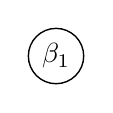
\begin{tikzpicture}
\node at (0, 0) [
  circle,                     % rectangle/diamond
  draw          = black,      % border
  line width    = .5pt,       % border width
  minimum size  = 20pt,       % minimum size of node
  inner sep     = 1pt,        % sep b/w border and inner text
  font          = \normalsize,%
  text          = black,      % inner label color
  fill          = white,
  node distance = 1pt,
  ]
  (beta1)
  {\( \beta_{1}  \)} ;
\end{tikzpicture}
\end{figure}
\end{lstlisting}

\begin{figure}[ht]\centering
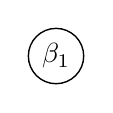
\begin{tikzpicture}
\node at (0, 0) [
  circle,                     % rectangle/diamond
  draw          = black,      % border
  line width    = .5pt,       % border width
  minimum size  = 20pt,       % minimum size of node
  inner sep     = 1pt,        % sep b/w border and inner text
  font          = \normalsize,%
  text          = black,      % inner label color
  fill          = white,
  node distance = 1pt,
  ]
  (beta1)
  {\( \beta_{1}  \)} ;
\end{tikzpicture}
\end{figure}


\lstset{numbers=left,language=[LaTeX]TeX,label= ,caption= ,captionpos=b}
\begin{lstlisting}
\begin{figure}[ht]\centering
\begin{tikzpicture}
\node at (0, 0) [
  circle,                     % rectangle/diamond
  draw          = black,      % border
  line width    = .5pt,       % border width
  minimum size  = 20pt,       % minimum size of node
  inner sep     = 1pt,        % sep b/w border and inner text
  font          = \normalsize,%
  text          = black,      % inner label color
  fill          = white,
  node distance = 1pt,
  ]
  (beta1)
  {\( \beta_{1}  \)} ; %
\node at (1, 0) [
  circle,                     % rectangle/diamond
  draw          = black,      % border
  ]
  ()
  {\( \Sigma  \)} ;
\node at (3, 0) [latent ] (id) {<label>} ; %
\node at (5, 0) [obs    ] (mu) {\( \mu  \)} ; %
\node at (7, 0) [const  ] (id-x) {X} ; %
\end{tikzpicture}
\end{figure}
\end{lstlisting}

\begin{figure}[ht]\centering
\begin{tikzpicture}
\node at (0, 0) [
  circle,                     % rectangle/diamond
  draw          = black,      % border
  line width    = .5pt,       % border width
  minimum size  = 20pt,       % minimum size of node
  inner sep     = 1pt,        % sep b/w border and inner text
  font          = \normalsize,%
  text          = black,      % inner label color
  fill          = white,
  node distance = 1pt,
  ]
  (beta1)
  {\( \beta_{1}  \)} ; %
\node at (1, 0) [
  circle,                     % rectangle/diamond
  draw          = black,      % border
  ]
  ()
  {\( \Sigma  \)} ;
\node at (3, 0) [latent ] (id) {<label>} ; %
\node at (5, 0) [obs    ] (mu) {\( \mu  \)} ; %
\node at (7, 0) [const  ] (id-x) {X} ; %
\end{tikzpicture}
\end{figure}



\FloatBarrier
\clearpage
\section{Plate and Parametric Models}
\label{sec:org5bdfec1}

\subsection{Basic shapes}
\label{sec:org59145b7}

\begin{figure}[ht]\centering
\begin{tikzpicture}
\node at (0, 0) [latent ] (a) {a} ; %
\node at (2, 0) [latent ] (b) {b} ; %
\node at (4, 1) [latent ] (c) {c} ; %
\node at (6, 1) [latent ] (d) {d} ; %
\node at (2,-1) [latent ] (e) {e} ; %
%% 
\plate [solid]   {plate1} {(e) (b)} {}; %
\plate [dashed]  {plate2} {(a) (c)} {\( i=1,..., n \)}; %
\plate [dotted]  {plate3} {(c) (d)} {N}; %
\end{tikzpicture}
\end{figure}


\subsection{Examples}
\label{sec:org120b2d9}

\lstset{numbers=left,language=[LaTeX]TeX,label= ,caption= ,captionpos=b}
\begin{lstlisting}
\begin{figure}[ht]\centering
\begin{tikzpicture}[thick,scale=1, every node/.style={transform shape}]
%% Nodes
\node at (2, 0) [obs        ] (yi)         {\( y_i \)} ; %
\node at (0, 0) [latent     ] (fi)         {\( f_i \)} ; %
\node at (-2, 0) [latent    ] (betai)      {\( \beta_ {i}  \)} ; %
\node at (-2, 2) [const     ] (Sigmabeta)  {\( \Sigma_{\beta }  \)} ; %
\node at (-4, 0) [const    ] (mubeta)     {\( \mu_   {\beta }  \)} ; %
\node at (0, 2) [latent     ] (theta)      {\( \theta  \)} ; %
\node at (-1, 4) [const     ] (mutheta)    {\( \mu_   {\theta } =0 \)} ; %
\node at ( 1, 4) [const     ] (Sigmatheta) {\( \Sigma_{\theta }=I   \)} ; %
\node at (-1, -2.5) [const  ] (l)          {\( l=1 \)} ; %
\node at ( 1, -2.5) [const  ] (sigmaf)     {\( \sigma_{f} =1 \)} ; %

%% plate
\plate {plate1} {(betai) (fi) (yi)} {\( i=1,...n \)}; 

%% arrows
\edgesimple {fi} {yi}
\edgesimple {betai} {fi}
\edgesimple {mubeta} {betai}
\edgesimple {l} {fi}
\edgesimple {sigmaf} {fi}
\edgesimple {Sigmabeta} {betai}
\edgesimple {mutheta} {theta}
\edgesimple {Sigmatheta} {theta}
\edgesimple {theta} {fi}
\end{tikzpicture}
\end{figure}
\end{lstlisting}

\begin{figure}[ht]\centering
\begin{tikzpicture}[thick,scale=1, every node/.style={transform shape}]
%% Nodes
\node at (2, 0) [obs        ] (yi)         {\( y_i \)} ; %
\node at (0, 0) [latent     ] (fi)         {\( f_i \)} ; %
\node at (-2, 0) [latent    ] (betai)      {\( \beta_ {i}  \)} ; %
\node at (-2, 2) [const     ] (Sigmabeta)  {\( \Sigma_{\beta }  \)} ; %
\node at (-4, 0) [const    ] (mubeta)     {\( \mu_   {\beta }  \)} ; %
\node at (0, 2) [latent     ] (theta)      {\( \theta  \)} ; %
\node at (-1, 4) [const     ] (mutheta)    {\( \mu_   {\theta } =0 \)} ; %
\node at ( 1, 4) [const     ] (Sigmatheta) {\( \Sigma_{\theta }=I   \)} ; %
\node at (-1, -2.5) [const  ] (l)          {\( l=1 \)} ; %
\node at ( 1, -2.5) [const  ] (sigmaf)     {\( \sigma_{f} =1 \)} ; %

%% plate
\plate {plate1} {(betai) (fi) (yi)} {\( i=1,...n \)}; 

%% arrows
\edgesimple {fi} {yi}
\edgesimple {betai} {fi}
\edgesimple {mubeta} {betai}
\edgesimple {l} {fi}
\edgesimple {sigmaf} {fi}
\edgesimple {Sigmabeta} {betai}
\edgesimple {mutheta} {theta}
\edgesimple {Sigmatheta} {theta}
\edgesimple {theta} {fi}
\end{tikzpicture}
\end{figure}


\lstset{numbers=left,language=[LaTeX]TeX,label= ,caption= ,captionpos=b}
\begin{lstlisting}
\begin{figure}[ht]\centering
\begin{tikzpicture}[thick,scale=1, every node/.style={transform shape}, on grid, auto]
%% Nodes
\node at (-6, 0) [const                ] (mubeta)      {\( \mu_   {\beta }  \)} ; %
\node at (-4, 2) [const                ] (Sigmabeta)  {\( \Sigma_{\beta }  \)} ; %
\node at (-4, 0) [dist, label={[red    ]below:\normalsize\( \No \)}  ] (normal)  {} ; %
\node at (2, 0) [obs                   ] (yi)         {\( y_i \)} ; %
\node at (0, 0) [latent                ] (fi)         {\( f_i \)} ; %
\node at (-2, 0) [latent               ] (betai)      {\( \beta_ {i}  \)} ; %
\node at (0, 2) [latent                ] (theta)      {\( \theta  \)} ; %
\node at (-1, 5) [const                ] (mutheta)    {\( \mu_   {\theta } =0 \)} ; %
\node at ( 1, 5) [const                ] (Sigmatheta) {\( \Sigma_{\theta }	=I   \)} ; %
\node at (-1, -4) [const             ] (l)          {\( l				=1 \)} ; %
\node at ( 1, -4) [const             ] (sigmaf)     {\( \sigma_{f}		=1 \)} ; %
\node at (0, -2.5) [dist, label={[black]right:\normalsize \( \G \)}  ] (g)  {} ; % 
\node at (2, 2) [operation             ] (dot) {\( \norm{.}   \)} ; %
\node at (4, 3) [latent                ] (x) {\( X \)} ; %
\node at (4, 1) [latent                ] (z) {\( Z \)} ; %
\node at (0, 3.5) [dist, label={[black]right:\normalsize\( \No \)}  ] (normaltheta)  {} ; % 
%% arrows
\edgesimple [-] {mubeta} {normal}
\edgesimple [-] {Sigmabeta} {normal}
\edgesimple {normal} {betai} ;
\edgesimple {fi} {yi}
\edgesimple {betai} {fi}
\edgesimple [-] {l} {g}
\edgesimple [-] {sigmaf} {g}
\edgesimple {g} {fi} ;
\edgesimple [-] {mutheta} {normaltheta}
\edgesimple [-] {Sigmatheta} {normaltheta}
\edgesimple {normaltheta} {theta} ;
\edgesimple {theta} {fi}
\edgesimple [-] {x} {dot} ;
\edgesimple [-] {z} {dot} ;
\edgesimple {dot} {theta} ;

%% plate
\plate {plate1} {(betai) (fi) (yi)} {\( i=1,...n \)}; 
\end{tikzpicture}
\end{figure}
\end{lstlisting}

\begin{figure}[ht]\centering
\begin{tikzpicture}[thick,scale=1, every node/.style={transform shape}, on grid, auto]
%% Nodes
\node at (-6, 0) [const                ] (mubeta)      {\( \mu_   {\beta }  \)} ; %
\node at (-4, 2) [const                ] (Sigmabeta)  {\( \Sigma_{\beta }  \)} ; %
\node at (-4, 0) [dist, label={[red    ]below:\normalsize\( \No \)}  ] (normal)  {} ; %
\node at (2, 0) [obs                   ] (yi)         {\( y_i \)} ; %
\node at (0, 0) [latent                ] (fi)         {\( f_i \)} ; %
\node at (-2, 0) [latent               ] (betai)      {\( \beta_ {i}  \)} ; %
\node at (0, 2) [latent                ] (theta)      {\( \theta  \)} ; %
\node at (-1, 5) [const                ] (mutheta)    {\( \mu_   {\theta } =0 \)} ; %
\node at ( 1, 5) [const                ] (Sigmatheta) {\( \Sigma_{\theta }	=I   \)} ; %
\node at (-1, -4) [const             ] (l)          {\( l				=1 \)} ; %
\node at ( 1, -4) [const             ] (sigmaf)     {\( \sigma_{f}		=1 \)} ; %
\node at (0, -2.5) [dist, label={[black]right:\normalsize \( \G \)}  ] (g)  {} ; % 
\node at (2, 2) [operation             ] (dot) {\( \norm{.}   \)} ; %
\node at (4, 3) [latent                ] (x) {\( X \)} ; %
\node at (4, 1) [latent                ] (z) {\( Z \)} ; %
\node at (0, 3.5) [dist, label={[black]right:\normalsize\( \No \)}  ] (normaltheta)  {} ; % 
%% arrows
\edgesimple [-] {mubeta} {normal}
\edgesimple [-] {Sigmabeta} {normal}
\edgesimple {normal} {betai} ;
\edgesimple {fi} {yi}
\edgesimple {betai} {fi}
\edgesimple [-] {l} {g}
\edgesimple [-] {sigmaf} {g}
\edgesimple {g} {fi} ;
\edgesimple [-] {mutheta} {normaltheta}
\edgesimple [-] {Sigmatheta} {normaltheta}
\edgesimple {normaltheta} {theta} ;
\edgesimple {theta} {fi}
\edgesimple [-] {x} {dot} ;
\edgesimple [-] {z} {dot} ;
\edgesimple {dot} {theta} ;

%% plate
\plate {plate1} {(betai) (fi) (yi)} {\( i=1,...n \)}; 
\end{tikzpicture}
\end{figure}

\section{DAG}
\label{sec:org6f9a3bb}
\subsection{Nodes as Text and box}
\label{sec:org7b60d49}
\lstset{numbers=left,language=[LaTeX]TeX,label= ,caption= ,captionpos=b}
\begin{lstlisting}
\begin{figure}[ht]\centering
\begin{tikzpicture}[thick,scale=1, every node/.style={transform shape}, on grid, auto]
\node at (0, 0)   [textnode, text width=2.5cm    ] (ind) {Socio-economic Positions} ; %
\node at (2.5, 2) [textnode, text width=1.8cm    ] (med) {Perceptions} ; %
\node at (5, 0)   [textnode, text width=2cm    ] (out) {Support for Populism} ; %

%% edges
\path[->] (ind)  edge node[el,left,rotate=0] {\( \lambda \quad \) }   (med);
\path[->] (med)  edge node[el,right,rotate=0] {\(\quad \beta  \)}   (out);
\path[->] (ind)  edge node[el,above,rotate=0] {\( \alpha  \)}   (out);
\end{tikzpicture}
\end{figure}
\end{lstlisting}

\begin{figure}[ht]\centering
\begin{tikzpicture}[thick,scale=1, every node/.style={transform shape}, on grid, auto]
\node at (0, 0)   [textnode, text width=2.5cm    ] (ind) {Socio-economic Positions} ; %
\node at (2.5, 2) [textnode, text width=1.8cm    ] (med) {Perceptions} ; %
\node at (5, 0)   [textnode, text width=2cm    ] (out) {Support for Populism} ; %

%% edges
\path[->] (ind)  edge node[el,left,rotate=0] {\( \lambda \quad \) }   (med);
\path[->] (med)  edge node[el,right,rotate=0] {\(\quad \beta  \)}   (out);
\path[->] (ind)  edge node[el,above,rotate=0] {\( \alpha  \)}   (out);
\end{tikzpicture}
\end{figure}

\subsection{Nodes as text}
\label{sec:orgfb6d91a}

\lstset{numbers=left,language=[LaTeX]TeX,label= ,caption= ,captionpos=b}
\begin{lstlisting}
\begin{figure}[ht]\centering
\begin{tikzpicture}[thick,scale=1, every node/.style={transform shape}, on grid, auto]
\node at (0, 0)   [text width=2.5cm    ] (ind) {Socio-economic Positions} ; %
\node at (2.5, 2) [text width=1.8cm    ] (med) {Perceptions} ; %
\node at (5, 0)   [text width=2cm    ] (out) {Support for Populism} ; %

%% edges
\path[->] (ind)  edge node[el,left,rotate=0] {\( \lambda \quad \) }   (med);
\path[->] (med)  edge node[el,right,rotate=0] {\(\quad \beta  \)}   (out);
\path[->] (ind)  edge node[el,above,rotate=0] {\( \alpha  \)}   (out);
\end{tikzpicture}
\end{figure}
\end{lstlisting}

\begin{figure}[ht]\centering
\begin{tikzpicture}[thick,scale=1, every node/.style={transform shape}, on grid, auto]
\node at (0, 0)   [text width=2.5cm    ] (ind) {Socio-economic Positions} ; %
\node at (2.5, 2) [text width=1.8cm    ] (med) {Perceptions} ; %
\node at (5, 0)   [text width=2cm    ] (out) {Support for Populism} ; %

%% edges
\path[->] (ind)  edge node[el,left,rotate=0] {\( \lambda \quad \) }   (med);
\path[->] (med)  edge node[el,right,rotate=0] {\(\quad \beta  \)}   (out);
\path[->] (ind)  edge node[el,above,rotate=0] {\( \alpha  \)}   (out);
\end{tikzpicture}
\end{figure}

\subsection{Nodes as variables (relative position)}
\label{sec:org4a477aa}

\lstset{numbers=left,language=[LaTeX]TeX,label= ,caption= ,captionpos=b}
\begin{lstlisting}
\begin{figure}[ht]\centering
\begin{tikzpicture}[thick,scale=1, every node/.style={transform shape}, on grid, auto]
\node at (0, 0)   [   ] (ind) {X} ; %
\node (med) [above right =  1.5cm and 1.5cm of ind] {Z};
\node (out) [right = 3cm and 3cm of ind] {Y} ; %

%% edges
\path[->] (ind)  edge node[el,left,rotate=0] {\( \lambda \quad \) }   (med);
\path[->] (med)  edge node[el,right,rotate=0] {\(\quad \beta  \)}   (out);
\path[->] (ind)  edge node[el,above,rotate=0] {\( \alpha  \)}   (out);
\end{tikzpicture}
\end{figure}
\end{lstlisting}

\begin{figure}[ht]\centering
\begin{tikzpicture}[thick,scale=1, every node/.style={transform shape}, on grid, auto]
\node at (0, 0)   [   ] (ind) {X} ; %
\node (med) [above right =  1.5cm and 1.5cm of ind] {Z};
\node (out) [right = 3cm and 3cm of ind] {Y} ; %

%% edges
\path[->] (ind)  edge node[el,left,rotate=0] {\( \lambda \quad \) }   (med);
\path[->] (med)  edge node[el,right,rotate=0] {\(\quad \beta  \)}   (out);
\path[->] (ind)  edge node[el,above,rotate=0] {\( \alpha  \)}   (out);
\end{tikzpicture}
\end{figure}

\subsection{Nodes as variables and circles}
\label{sec:orge5bcee8}

\lstset{numbers=left,language=[LaTeX]TeX,label= ,caption= ,captionpos=b}
\begin{lstlisting}
\begin{figure}[ht]\centering
\begin{tikzpicture}[thick,scale=1, every node/.style={transform shape}, on grid, auto]
\node at (0, 0)   [latent     ] (ind) {X} ; %
\node at (2.5, 2) [latent,    ] (med) {Z} ; %
\node at (5, 0)   [latent,    ] (out) {Y} ; %

%% edges
\path[->] (ind)  edge node[el,left,rotate=0] {\( \lambda \quad \) }   (med);
\path[->] (med)  edge node[el,right,rotate=0] {\(\quad \beta  \)}   (out);
\path[->] (ind)  edge node[el,above,rotate=0] {\( \alpha  \)}   (out);
\end{tikzpicture}
\end{figure}
\end{lstlisting}

\begin{figure}[ht]\centering
\begin{tikzpicture}[thick,scale=1, every node/.style={transform shape}, on grid, auto]
\node at (0, 0)   [latent     ] (ind) {X} ; %
\node at (2.5, 2) [latent,    ] (med) {Z} ; %
\node at (5, 0)   [latent,    ] (out) {Y} ; %

%% edges
\path[->] (ind)  edge node[el,left,rotate=0] {\( \lambda \quad \) }   (med);
\path[->] (med)  edge node[el,right,rotate=0] {\(\quad \beta  \)}   (out);
\path[->] (ind)  edge node[el,above,rotate=0] {\( \alpha  \)}   (out);
\end{tikzpicture}
\end{figure}


\subsection{Nodes as variables and circles (closer)}
\label{sec:orgf822513}


\lstset{numbers=left,language=[LaTeX]TeX,label= ,caption= ,captionpos=b}
\begin{lstlisting}
\begin{figure}[ht]\centering
\begin{tikzpicture}[thick,scale=1, every node/.style={transform shape}, on grid, auto]
\node at (0, 0)   [latent     ] (ind) {X} ; %
\node at (2, 1.5) [latent,    ] (med) {Z} ; %
\node at (4, 0)   [latent,    ] (out) {Y} ; %

%% edges
\path[->] (ind)  edge node[el,left,rotate=0] {\( \lambda \quad \) }   (med);
\path[->] (med)  edge node[el,right,rotate=0] {\(\quad \beta  \)}   (out);
\path[->] (ind)  edge node[el,above,rotate=0] {\( \alpha  \)}   (out);
\end{tikzpicture}
\end{figure}
\end{lstlisting}

\begin{figure}[ht]\centering
\begin{tikzpicture}[thick,scale=1, every node/.style={transform shape}, on grid, auto]
\node at (0, 0)   [latent     ] (ind) {X} ; %
\node at (2, 1.5) [latent,    ] (med) {Z} ; %
\node at (4, 0)   [latent,    ] (out) {Y} ; %

%% edges
\path[->] (ind)  edge node[el,left,rotate=0] {\( \lambda \quad \) }   (med);
\path[->] (med)  edge node[el,right,rotate=0] {\(\quad \beta  \)}   (out);
\path[->] (ind)  edge node[el,above,rotate=0] {\( \alpha  \)}   (out);
\end{tikzpicture}
\end{figure}


\subsection{Nodes as variables and circles (closer, no edge labels)}
\label{sec:orga30954e}


\lstset{numbers=left,language=[LaTeX]TeX,label= ,caption= ,captionpos=b}
\begin{lstlisting}
\begin{figure}[ht]\centering
\begin{tikzpicture}[thick,scale=1, every node/.style={transform shape}, on grid, auto]
\node at (0, 0)   [latent     ] (ind) {X} ; %
\node at (2, 1.5) [latent,    ] (med) {Z} ; %
\node at (4, 0)   [latent,    ] (out) {Y} ; %

%% edges
\path[->] (ind)  edge node[el,left,rotate=0]  {}   (med);
\path[->] (med)  edge node[el,right,rotate=0] {}   (out);
\path[->] (ind)  edge node[el,above,rotate=0] {}   (out);
\end{tikzpicture}
\end{figure}
\end{lstlisting}

\begin{figure}[ht]\centering
\begin{tikzpicture}[thick,scale=1, every node/.style={transform shape}, on grid, auto]
\node at (0, 0)   [latent     ] (ind) {X} ; %
\node at (2, 1.5) [latent,    ] (med) {Z} ; %
\node at (4, 0)   [latent,    ] (out) {Y} ; %

%% edges
\path[->] (ind)  edge node[el,left,rotate=0]  {}   (med);
\path[->] (med)  edge node[el,right,rotate=0] {}   (out);
\path[->] (ind)  edge node[el,above,rotate=0] {}   (out);
\end{tikzpicture}
\end{figure}

\subsection{Nodes as variables and circles (closer, no edge labels, and subfigures)}
\label{sec:org33606e4}

\lstset{numbers=left,language=[LaTeX]TeX,label= ,caption= ,captionpos=b}
\begin{lstlisting}
\begin{figure}[ht]
\begin{subfigure}{.5\textwidth}
  % ------------------------------
  \centering
  \begin{tikzpicture}[thick,scale=1, every node/.style={transform shape}, on grid, auto]
  \node at (0, 0)   [latent     ] (ind) {X} ; %
  \node at (2, 1.5) [latent,    ] (med) {Z} ; %
  \node at (4, 0)   [latent,    ] (out) {Y} ; %
  
  %% edges
  \path[->] (ind)  edge node[el,left,rotate=0]  {}   (med);
  \path[->] (med)  edge node[el,right,rotate=0] {}   (out);
  \path[->] (ind)  edge node[el,above,rotate=0] {}   (out);
  \end{tikzpicture}
  \caption{Put your sub-caption here}
  \label{fig:sub-first}
  % ------------------------------
\end{subfigure}
\begin{subfigure}{.5\textwidth}
  % ------------------------------
  \centering
  \begin{tikzpicture}[thick,scale=.7, every node/.style={transform shape}, on grid, auto]
  \node at (0, 0)   [latent     ] (ind) {X} ; %
  \node at (2, 1.5) [latent,    ] (med) {Z} ; %
  \node at (4, 0)   [latent,    ] (out) {Y} ; %
  
  %% edges
  \path[->] (ind)  edge node[el,left,rotate=0]  {}   (med);
  \path[<-] (med)  edge node[el,right,rotate=0] {}   (out);
  \path[->] (ind)  edge node[el,above,rotate=0] {}   (out);
  \end{tikzpicture}
  \caption{Put your sub-caption here}
  \label{fig:sub-second}
  % ------------------------------
\end{subfigure}
\caption{Put your caption here}
\label{fig:fig}
\end{figure}
\end{lstlisting}

\begin{figure}[ht]
\begin{subfigure}{.5\textwidth}
  % ------------------------------
  \centering
  \begin{tikzpicture}[thick,scale=1, every node/.style={transform shape}, on grid, auto]
  \node at (0, 0)   [latent     ] (ind) {X} ; %
  \node at (2, 1.5) [latent,    ] (med) {Z} ; %
  \node at (4, 0)   [latent,    ] (out) {Y} ; %
  
  %% edges
  \path[->] (ind)  edge node[el,left,rotate=0]  {}   (med);
  \path[->] (med)  edge node[el,right,rotate=0] {}   (out);
  \path[->] (ind)  edge node[el,above,rotate=0] {}   (out);
  \end{tikzpicture}
  \caption{Put your sub-caption here}
  \label{fig:sub-first}
  % ------------------------------
\end{subfigure}
\begin{subfigure}{.5\textwidth}
  % ------------------------------
  \centering
  \begin{tikzpicture}[thick,scale=.7, every node/.style={transform shape}, on grid, auto]
  \node at (0, 0)   [latent     ] (ind) {X} ; %
  \node at (2, 1.5) [latent,    ] (med) {Z} ; %
  \node at (4, 0)   [latent,    ] (out) {Y} ; %
  
  %% edges
  \path[->] (ind)  edge node[el,left,rotate=0]  {}   (med);
  \path[<-] (med)  edge node[el,right,rotate=0] {}   (out);
  \path[->] (ind)  edge node[el,above,rotate=0] {}   (out);
  \end{tikzpicture}
  \caption{Put your sub-caption here}
  \label{fig:sub-second}
  % ------------------------------
\end{subfigure}
\caption{Put your caption here}
\label{fig:fig}
\end{figure}

\subsection{Large DAG}
\label{sec:org1adab87}

\begin{figure}[ht]\centering
\begin{tikzpicture}[thick,scale=1, every node/.style={transform shape}, on grid, auto]
\node at (0, 0) [] (x) {X} ;
\node[above right = 1.5cm and 1.5cm of x] (z) {Z};
\node[right = 3cm and 3cm of x] (y) {Y};
\node[above left = 1.5cm and 1.5cm of x] (u1) {\( U_1 \)};
\node[above right = 1.5cm and 1.5cm of u1] (u2) {\( U_2 \)};
%% edges
\edgesimple {x} {y} ;
\edgesimple {x} {z} ;
\edgesimple {z} {y} ;
\edgesimple {u1} {z} ;
\edgesimple {u2} {z} ;
\edgesimple {u2} {u1} ;
\edgesimple {u1} {x} ;
\end{tikzpicture}
\end{figure}


\subsection{Large DAG (using latent var notation)}
\label{sec:org7b75cf7}

\begin{figure}[ht]\centering
\begin{tikzpicture}[thick,scale=1, every node/.style={transform shape}, on grid, auto]
\node at (0, 0) [obs] (x) {X} ;
\node[obs, above right = 1.5cm and 1.5cm of x] (z) {Z};
\node[obs, right = 3cm and 3cm of x] (y) {Y};
\node[latent, above left = 1.5cm and 1.5cm of x] (u1) {\( U_1 \)};
\node[latent, above right = 1.5cm and 1.5cm of u1] (u2) {\( U_2 \)};
%% edges
\edgesimple {x} {y} ;
\edgesimple {x} {z} ;
\edgesimple {z} {y} ;
\edgesimple {u1} {z} ;
\edgesimple {u2} {z} ;
\edgesimple {u2} {u1} ;
\edgesimple {u1} {x} ;
\end{tikzpicture}
\end{figure}


\subsection{Large DAG (using latent var notation alternative)}
\label{sec:org2d50678}


\begin{figure}[ht]\centering
\begin{tikzpicture}[thick,scale=1, every node/.style={transform shape}, on grid, auto]
\node at (0, 0) [latent] (x) {X} ;
\node[latent, above right = 1.5cm and 1.5cm of x] (z) {Z};
\node[latent, right = 3cm and 3cm of x] (y) {Y};
\node[latent, dashed, above left = 1.5cm and 1.5cm of x] (u1) {\( U_1 \)};
\node[latent, dashed, above right = 1.5cm and 1.5cm of u1] (u2) {\( U_2 \)};
%% edges
\edgesimple {x} {y} ;
\edgesimple {x} {z} ;
\edgesimple {z} {y} ;
\edgesimple {u1} {z} ;
\edgesimple {u2} {z} ;
\edgesimple {u2} {u1} ;
\edgesimple {u1} {x} ;
\end{tikzpicture}
\end{figure}

\section{Undirected Graphs}
\label{sec:org5c7e0bf}

\lstset{numbers=left,language=[LaTeX]TeX,label= ,caption= ,captionpos=b}
\begin{lstlisting}
\begin{figure}[ht]
\scalebox{.75}{ % to reduce the size of the figure (package graphix)
% nodes: latent, obs, det, const, factor, plate, gate
\centering
\tikz{ %
\node[latent] (x1) {\( X_1 \)} ; %
\node[latent, right=of x1] (x2) {\( X_2 \)} ; %
\node[latent, right=of x2] (x3) {\( X_3 \)} ; %
\node[latent, above=of x3] (x4) {\( X_4 \)} ; %
\edgesimple [-] {x1} {x2} ; %
\edgesimple [-] {x2} {x3} ; %
\edgesimple [-] {x3} {x4} ; %
\edgesimple [-] {x2} {x4} ; %
\edgesimple[bend right, -] {x1} {x3} ; %
}
~~~~
\tikz{ %
\node[latent] (x1) {\( X_1 \)} ; %
\node[latent, right=of x1] (x2) {\( X_2 \)} ; %
\node[latent, right=of x2] (x3) {\( X_3 \)} ; %
\node[latent, right=of x3] (x4) {\( X_4 \)} ; %
% second row
\node[latent, below=of x1] (x5) {\( X_5 \)} ; %
\node[latent, below=of x2] (x6) {\( X_6 \)} ; %
\node[latent, below=of x3] (x7) {\( X_7 \)} ; %
\node[latent, below=of x4] (x8) {\( X_8 \)} ; %
% third row
\node[latent, below=of x5] (x9) {\( X_9 \)} ; %
\node[latent, below=of x6] (x10) {\( X_{10} \)} ; %
\node[latent, below=of x7] (x11) {\( X_{11} \)} ; %
\node[latent, below=of x8] (x12) {\( X_{12} \)} ; %
\edgesimple [-] {x1} {x2} ; %
\edgesimple [-] {x2} {x3} ; %
\edgesimple [-] {x3} {x4} ; %
\edgesimple [-] {x1} {x5} ; %
\edgesimple [-] {x2} {x6} ; %
\edgesimple [-] {x3} {x7} ; %
\edgesimple [-] {x4} {x8} ; %
\edgesimple [-] {x5} {x6} ; %
\edgesimple [-] {x6} {x7} ; %
\edgesimple [-] {x7} {x8} ; %
\edgesimple [-] {x5} {x9} ; %
\edgesimple [-] {x6} {x10} ; %
\edgesimple [-] {x7} {x11} ; %
\edgesimple [-] {x8} {x12} ; %
\edgesimple [-] {x9} {x10} ; %
\edgesimple [-] {x10} {x11} ; %
\edgesimple [-] {x11} {x12} ; %
}
}
\end{figure}
\end{lstlisting}

\begin{figure}[ht]
\scalebox{.75}{ % to reduce the size of the figure (package graphix)
% nodes: latent, obs, det, const, factor, plate, gate
\centering
\tikz{ %
\node[latent] (x1) {\( X_1 \)} ; %
\node[latent, right=of x1] (x2) {\( X_2 \)} ; %
\node[latent, right=of x2] (x3) {\( X_3 \)} ; %
\node[latent, above=of x3] (x4) {\( X_4 \)} ; %
\edgesimple [-] {x1} {x2} ; %
\edgesimple [-] {x2} {x3} ; %
\edgesimple [-] {x3} {x4} ; %
\edgesimple [-] {x2} {x4} ; %
\edgesimple[bend right, -] {x1} {x3} ; %
}
~~~~
\tikz{ %
\node[latent] (x1) {\( X_1 \)} ; %
\node[latent, right=of x1] (x2) {\( X_2 \)} ; %
\node[latent, right=of x2] (x3) {\( X_3 \)} ; %
\node[latent, right=of x3] (x4) {\( X_4 \)} ; %
% second row
\node[latent, below=of x1] (x5) {\( X_5 \)} ; %
\node[latent, below=of x2] (x6) {\( X_6 \)} ; %
\node[latent, below=of x3] (x7) {\( X_7 \)} ; %
\node[latent, below=of x4] (x8) {\( X_8 \)} ; %
% third row
\node[latent, below=of x5] (x9) {\( X_9 \)} ; %
\node[latent, below=of x6] (x10) {\( X_{10} \)} ; %
\node[latent, below=of x7] (x11) {\( X_{11} \)} ; %
\node[latent, below=of x8] (x12) {\( X_{12} \)} ; %
\edgesimple [-] {x1} {x2} ; %
\edgesimple [-] {x2} {x3} ; %
\edgesimple [-] {x3} {x4} ; %
\edgesimple [-] {x1} {x5} ; %
\edgesimple [-] {x2} {x6} ; %
\edgesimple [-] {x3} {x7} ; %
\edgesimple [-] {x4} {x8} ; %
\edgesimple [-] {x5} {x6} ; %
\edgesimple [-] {x6} {x7} ; %
\edgesimple [-] {x7} {x8} ; %
\edgesimple [-] {x5} {x9} ; %
\edgesimple [-] {x6} {x10} ; %
\edgesimple [-] {x7} {x11} ; %
\edgesimple [-] {x8} {x12} ; %
\edgesimple [-] {x9} {x10} ; %
\edgesimple [-] {x10} {x11} ; %
\edgesimple [-] {x11} {x12} ; %
}
}
\end{figure}


\section{Tree}
\label{sec:orgcef8052}

It uses the package \texttt{forest}, so you need to include \texttt{\textbackslash{}usepackage\{forest\}} in the latex header.
Snippet: dagtree


\lstset{numbers=left,language=[LaTeX]TeX,label= ,caption= ,captionpos=b}
\begin{lstlisting}
\begin{figure}[ht]\centering
\begin{forest}
  % for tree={l+=1cm} % increase level distance
  [root
    [left[lleft][lright]]
    [left[lleft][lright]]
    [\( \cdots  \)]
    [right[rleft][rright[leaf left][leaf right]]]
  ]
\end{forest}
\end{figure}
\end{lstlisting}

\begin{figure}[ht]\centering
\begin{forest}
  % for tree={l+=1cm} % increase level distance
  [root
    [left[lleft][lright]]
    [left[lleft][lright]]
    [\( \cdots  \)]
    [right[rleft][rright[leaf left][leaf right]]]
  ]
\end{forest}
\end{figure}

\lstset{numbers=left,language=[LaTeX]TeX,label= ,caption= ,captionpos=b}
\begin{lstlisting}
\begin{figure}[ht]\centering
\begin{forest}
  % for tree={l+=1cm} % increase level distance
  [root
    [left node[ another left][ another right]]
    [right node]
  ]
\end{forest}
\end{figure}
\end{lstlisting}

\begin{figure}[ht]\centering
\begin{forest}
  % for tree={l+=1cm} % increase level distance
  [root
    [left node[ another left][ another right]]
    [right node]
  ]
\end{forest}
\end{figure}
\end{document}
